\section{Proposed \arcName~Technique}
\label{sec:design}
    The \arcName~technique proposed here is based on a direct hash mapping of GUID values to in-network router IP addresses.  In contrast to well-known DHT schemes, such as Chord~\cite{chord_stoica}, Pastry~\cite{pastry_Rowstron}, Tapestry~\cite{tapestry_Zhao} or Beehive~\cite{Beehive_Ramasubramanian}, this approach assumes the participation of routers in the \arcName~scheme in terms of responding to update and query messages and storing the relevant GUID:NA table entries as required by the distributed protocol. Note that because routers have access to intra- and inter-domain routing tables, once an IP address is obtained from the hash operation, no further information is required to route the table entries to the selected router where the entry is to be stored.  In addition, with $k>1$ hash mappings of GUID to router IP address, co-location at the router makes it possible to look up routing table information to determine path length/cost to aid selection between multiple alternative table storage locations. 
    %We consider networks in which an individual user is associated with a globally unique, long-term stable and location independent name, called \emph{GUID} (i.e Globally Unique IDentifier), and a routable address, called \emph{locator}. The mapping of  a particular GUID to its locator is stored in a network entity called \emph{resolver}. The naming resolution service is responsible managing these resolvers and providing the associated address for given GUID.
    %Our key idea to achieve fast lookup, fast update propagation and high scalability (i.e.  billions of GUID-to-address mappings) is the use of consistent hashing to leverage the underlying routing structures. While our approach is applicable to any underlying routing structures, let us use that of current Internet to illustrate our design for the simplicity in explanation. We defer the discussion of the design for users that has multiple routable addresses (i.e multi-homing) until the section \ref{}. In addition, it is worth to note that we assume no constraint on the structure of GUID space (i.e it can be structured or flat).
    %In this section, we first describe the basic design followed by the discussion on challenges that the design opens up. We then present the design extension to address those challenges and the incremental deployment plan.    
    \subsection{Base design}
        \arcName~is moving away from a centralized control over name and address ownership, which forms a single root of global trust, to a fully distributed, hence highly scalable scheme. \arcName~utilizes underlying routing infrastructure to create a network consisting of globally distributed nodes. Participating nodes are routers acting as resolvers that store GUID to locator mappings. Candidate routers are those that have access to table of all prefixes that announced by all ASes. In the current Internet, such information is readily available for all BGP routers of every ASes. Hence, we assume all routes participate in our naming resolution infrastructure are BGP speakers that sharing the same view of a global prefix table, just as prefix table of today's BGP.  The three pieces of information of the prefix table used in our scheme are \emph{announced prefix block}, \emph{AS number} of the entity announcing that block, and \emph{next-hop address} to reach that AS.        
        
        Overall, GUID to locator resolution in \arcName~takes place as illustrated in figure~\ref{fig:base_design}. A client sends a lookup request with the desired GUID the border gateway router of its AS. The border gateway applies a predefined consistent hashing function on the GUID to map it down to the address space. Note that for better reliability and low latency, the gateway might apply K different hash functions to the GUID and get K resolver's dresses. We defer the detail discussion of K>1 to subsection \ref{subsub:replication}. In the case of Internet, hashed result of an GUID is a 32-bit IP address (or 128-bit number for IPv6). The border gateway then finds the \emph{longest prefix matched} to the hashed result in order to identify the resolvers'AS number. Once the AS number is identified, the resolver address of the GUID is nothing but the next-hop address to reach that AS. We note that up until this step, all computation are done locally (i.e., without communication to remote nodes) by client's border gateway. Hence it is fast and does not consume any network bandwidth.
        Next, the client's border gateway sends the request to the resolver's address found in the previous step. Upon receiving the query, the resolver performs local lookup for the requested GUID and sends the result back to the client's border gateway, which in turns forwards it back to the client. % TOO CRYPTIC, need more refine to make it easier to understand

        As mapping of GUID to locator is changed, GUID owner must issue an update request to the resolution infrastructure. The sequence of steps for GUID insertion and update are identical to that of querying process.

     \subsection{Technical challenges and solutions}
        %So far, we have presented the base design for the resolution service. However, the architecture is far from an applicable solution due to many issues. We elaborate those challenges in this subsection and extend the design to make it a complete solution, satisfying the goals set in section \ref{sec:introduction}.
        Next, we discuss the challenges in our design.
        \subsubsection{IP hole effect}
        \label{subsub:replication}

        The major advantage of our approach comparing to existing ones is the use of direct hashing from name to resolver address. While the technique produces the benefit of low latency naming look up and update since it only requires one overlay hop to reach the resolver, it suffers to the discontinuity of the address space. Since the hashed value of a GUID is equally distributed over address space, there is a probability that the hashed value falls into the address block that no organization have announced. We call the problem is \emph{IP hole effect}. % might need to change the name
        For example, in current Internet, while there are $2^{32}$ possible IP addresses for IPv4, only 86\% of them are allocated to organizations. The rest are reserved for various purposes including multicast, limited multicast, loopback address, broadcast, etc. Among those allocated address, only 63.7\% of them are announced by organizations. As the result, the percentage of announced IP address is only 55\%[cite IP hole data] over the whole 32-bit IP space, giving the probability for a hashed result falling into one of the unannounced address is 45\%.

        \arcName~ addresses the IP hole effect by having the border gateway applying a predefined hash function on GUID up to M times. If after M tries, the hashed result still falls into one of the unannounced addresses, then from the announced prefix table, we pick the announced IP address that has minimum \emph{IP distance} to the current hashed value. We use that IP address as hashed result. Given two k-bit addresses, A and B, their IP distance is defined as follow:
        \begin{center} $IP\_distance_{[A,B]} = \displaystyle\sum\limits_{i=0}^{i=k-1} |A_i - B_i|*2^{i}$ \end{center}
        We further define IP distance of an address to an address block is the minimum IP address of that address to all address in that block.
        Figure \ref{fig:rehashing} shows the probability of the hashed result falling into the IP holes as M increases. With M=10, the probability falls as low as 0.009. Algorithm \ref{alg:rehashing} which summarizes steps taken by the gateway guarantees that a valid hashed result always be found.
       {\footnotesize
        \begin{algorithm}
            \DontPrintSemicolon
            \SetAlFnt{\small\sf}
            \SetKwData{numbtry}{number\_of\_tries}
            \SetKwData{mindist}{min\_distance}
            \SetKwData{result}{result} %declare
            \SetKwFunction{lpm}{Longest\_Prefix\_Matching}
            \SetKwFunction{ipd}{IP\_distance}
            \SetKwFunction{Hash}{hash}
            \SetKwInOut{Input}{input}
            \SetKwInOut{Output}{output}
            \Input{GUID - the $GUID$ to be hashed \\ \hspace{0.5cm}$M$ - maximum number of rehashing}
            \Output{An address guaranteed to be found in prefix table}
            \BlankLine
            $\numbtry \leftarrow 0 ;$\;
            $\result \leftarrow \Hash{GUID};$\;
            \While{ ($\numbtry < M $)}{
                \If{\lpm{\result} $>$ 0}{
                \Return \result; //ended here if found\;
                }
                 {// no prefix was found}\;
                $\result \leftarrow \Hash{\result}; $\;
                $\numbtry \leftarrow \numbtry+1 ;$\;
            }
            //No match found after M hashes\;
            $\mindist \leftarrow 2^{32}$;\;
            \lForEach{prefix $i$ in the Prefix Table}{\;
               \If{\ipd{\result,prefix $i$} $<$ \mindist}{
                   \mindist $\leftarrow$ \ipd{\result to the prefix};\;
                }
            }
            \Return An address in the prefix that has \mindist\;
         \caption{Hashing GUID to address space} \label{alg:rehashing}
        \end{algorithm}
        }
        It is noteworthy that the hashing, rehashing and prefix matching processes are done locally by the border gateway. Hence it does not introduce any overhead to the network. As a side note, we envision that the IP hole problem will exist on any addressing scheme, not only on our current IP network, which makes our patch more widely applicable.

        \subsubsection{Replication}
        \label{subsub:replication}
        To enhance system's reliability and further reduce access latencies, we increase number of resolvers to be responsible for each mapping by having the border gateways perform K different hash functions at the time of update and query.
        \begin{figure}[h]
            \centering
            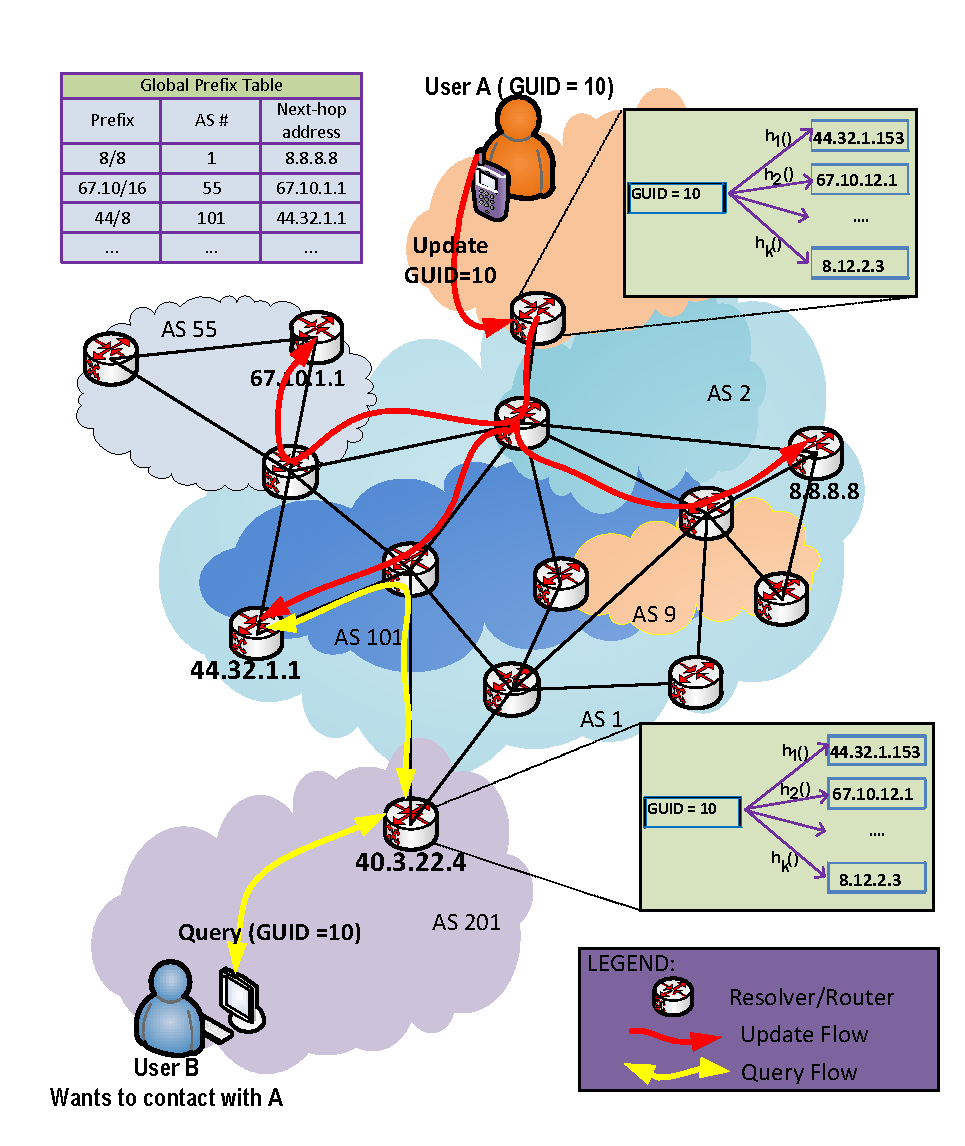
\includegraphics[width=0.5\textwidth]{figures/DirectHashingApproach.eps}
            \caption{An example of the update and query process with $K=3$ }
            \label{fig:design}
        \end{figure}
        After receiving the query, the border gateway applies Algorithm \ref{alg:rehashing} for K times with K different hashing functions to obtain K valid resolvers's addresses. Among these K resolver, It looks at the prefix table to choose the closest one. The notion of `closest' can be measure in terms of BGP distance (e.g. hop counts), or IP distance as mentioned in the previous subsection.

        Replicating the mapping can reduce access latencies and increase liability. Firstly, with replications, a gateway is more likely to find the closer resolver. We show in evaluation section, section \ref{sec:evaluation}, as K increases from 1 to 5, the 95 percentage lookup latency of the query is cut in half, from 202ms to 91ms with $K=5$. Secondly, as the number of replicas increases, the reliability of the system is also greatly improved as the probability of two distant routers to failure simultaneously is very low. Figure \ref{fig:design} illustrates an example of the update and query process with $K=3$. Lastly, we note that event with replication, no two routers share the same set of mappings. Hence, this interleaving replicas further increase system's reliability.
        %Having too many replica can leads to increase in update delay and introduce addional network traffic. As the result, we need to carefully choose value for K in our design.
        %While it is obvious to see the query latency reduces as higher K is used, K can not be arbitrarily increased due to update propagation delay. Specifically, propagation delay for each update equals to the largest update delay to individual resolver, assuming the gateway simultaneously updates to all resolvers at once. Hence the inherent trade of between query latency and update latency must be taken into account when K is being used as the knob to tuning the network's performance
        \subsubsection{Dynamism}
        \textbf{Change of announced prefix}:  Announced prefix changes occurred when an AS withdraws a previously announced prefix or announces a new prefix. In the former case, all mapping stored on that AS will neither be queried nor updated since it is not visible to other gateway, which we call them \emph{orphan mappings}. Keeping such mappings is wasting router's resource, which leads to the need of garbage collection. The AS can actively remove such orphan mappings by maintaining additional pointer for each mapping to identify prefix that the mapping belonging to based on which he know which mapping should be removed accordingly.

        For the planned withdrawing case, the AS can migrate all mappings he is hosting to the corresponding AS in the hashing chain. To do that, border gateway of that AS simply go over the list of GUID belong to the prefix to be removed that it stores, apply Algorithm \ref{alg:rehashing} to each GUID to get the valid resolvers' addresses excluding his own address. He then issues the GUID updates to those resolver addresses and delete his own copies of mappings. Upon finishing migration, the AS can withdraw the prefix safely. Note that for the security reason, all the updates must be verified. In particular, only GUID owner and AS on the hashing chain allowed to request mapping update for that GUID.

        In the latter case, where an AS announces new prefix, it becomes much more tricky. There will be queries that go to the AS with GUID that does not stored on any of the AS's border gateways, since it is stored in other AS that is behind the current AS in the hashing chain. In such cases, the border gateway of the newly announced AS has to (1) first verify that he is on the hash chain of of that GUID, which can be done simply by applying K hash functions, m times for each on the given GUID. After positively confirmed, (2) the border gateway must go the the address right after him on the hashing chain to get the GUID and (3) inform that the mapping now becomes orphan to the AS right behind him so that the behind AS can start collecting garbage, certainly after a verification. The border gateway then stores the mapping on to permanent memory in order to be ready for the next query of the same GUID. Note that to reduce the user visibility on prefix change, the border gateway can in parallel issues P query to P resolvers, with $P<K$.

        \textbf{Unreachable border gateway due to router failure} \arcName~is resilient to this type of dynamism by design. As failure of border gateway is made visible to other border
        of There must be timeout mechanism to detect the failure of resolver border gateway.

        \textbf{Simultaneous naming update and change in announced prefix} This will cause inconsistency in the returned locators if there are more than one entities request for the same GUID at the same time. Two users want to call to the same entity to start a 3-way conference call for example.

    \subsection{Incremental deployment plan}
        [Not sure if this section is needed. ]
        How the packet is modified, which flag need to be turned on..

        what need to be changed/ what need not to replace DNS (from application layer (socket binding), to TCP layer (query), to IP layer (IP packet header)...

